% Created 2024-11-04 Mon 00:46
% Intended LaTeX compiler: pdflatex
\documentclass[11pt]{article}
\usepackage[utf8]{inputenc}
\usepackage[T1]{fontenc}
\usepackage{graphicx}
\usepackage{longtable}
\usepackage{wrapfig}
\usepackage{rotating}
\usepackage[normalem]{ulem}
\usepackage{amsmath}
\usepackage{amssymb}
\usepackage{capt-of}
\usepackage{hyperref}
\usepackage[polish]{babel}
\usepackage[T1]{fontenc}
\usepackage[utf8]{inputenc}
\selectlanguage{polish}
\usepackage{caption}
\usepackage{booktabs}
\captionsetup{labelfont=bf}
\usepackage{float}
\usepackage[a4paper, total={6in, 8in}]{geometry}
\author{Piotr Karamon}
\date{04.11.2024r.}
\title{Laboratorium 4 - Producenci i konsumenci z losowa ilością pobieranych i wstawianych porcji}
\hypersetup{
 pdfauthor={Piotr Karamon},
 pdftitle={Laboratorium 4 - Producenci i konsumenci z losowa ilością pobieranych i wstawianych porcji},
 pdfkeywords={},
 pdfsubject={},
 pdfcreator={Emacs 29.2 (Org mode 9.7.11)}, 
 pdflang={Polish}}

% Setup for code blocks [1/2]

\usepackage{fvextra}

\fvset{%
  commandchars=\\\{\},
  highlightcolor=white!95!black!80!blue,
  breaklines=true,
  breaksymbol=\color{white!60!black}\tiny\ensuremath{\hookrightarrow}}

% Make line numbers smaller and grey.
\renewcommand\theFancyVerbLine{\footnotesize\color{black!40!white}\arabic{FancyVerbLine}}

\usepackage{xcolor}

% In case engrave-faces-latex-gen-preamble has not been run.
\providecolor{EfD}{HTML}{f7f7f7}
\providecolor{EFD}{HTML}{28292e}

% Define a Code environment to prettily wrap the fontified code.
\usepackage[breakable,xparse]{tcolorbox}
\DeclareTColorBox[]{Code}{o}%
{colback=EfD!98!EFD, colframe=EfD!95!EFD,
  fontupper=\footnotesize\setlength{\fboxsep}{0pt},
  colupper=EFD,
  IfNoValueTF={#1}%
  {boxsep=2pt, arc=2.5pt, outer arc=2.5pt,
    boxrule=0.5pt, left=2pt}%
  {boxsep=2.5pt, arc=0pt, outer arc=0pt,
    boxrule=0pt, leftrule=1.5pt, left=0.5pt},
  right=2pt, top=1pt, bottom=0.5pt,
  breakable}

% Support listings with captions
\usepackage{float}
\floatstyle{plain}
\newfloat{listing}{htbp}{lst}
\newcommand{\listingsname}{Listing}
\floatname{listing}{\listingsname}
\newcommand{\listoflistingsname}{List of Listings}
\providecommand{\listoflistings}{\listof{listing}{\listoflistingsname}}


% Setup for code blocks [2/2]: syntax highlighting colors

\newcommand\efstrut{\vrule height 2.1ex depth 0.8ex width 0pt}
\definecolor{EFD}{HTML}{000000}
\definecolor{EfD}{HTML}{ffffff}
\newcommand{\EFD}[1]{\textcolor{EFD}{#1}} % default
\newcommand{\EFvp}[1]{#1} % variable-pitch
\definecolor{EFh}{HTML}{595959}
\newcommand{\EFh}[1]{\textcolor{EFh}{#1}} % shadow
\definecolor{EFsc}{HTML}{005f5f}
\newcommand{\EFsc}[1]{\textcolor{EFsc}{\textbf{#1}}} % success
\definecolor{EFw}{HTML}{884900}
\newcommand{\EFw}[1]{\textcolor{EFw}{\textbf{#1}}} % warning
\definecolor{EFe}{HTML}{a60000}
\newcommand{\EFe}[1]{\textcolor{EFe}{\textbf{#1}}} % error
\definecolor{EFl}{HTML}{3548cf}
\newcommand{\EFl}[1]{\textcolor{EFl}{#1}} % link
\definecolor{EFlv}{HTML}{721045}
\newcommand{\EFlv}[1]{\textcolor{EFlv}{#1}} % link-visited
\definecolor{Efhi}{HTML}{b2e4dc}
\newcommand{\EFhi}[1]{\colorbox{Efhi}{\efstrut{}#1}} % highlight
\definecolor{EFc}{HTML}{595959}
\newcommand{\EFc}[1]{\textcolor{EFc}{\textit{#1}}} % font-lock-comment-face
\definecolor{EFcd}{HTML}{595959}
\newcommand{\EFcd}[1]{\textcolor{EFcd}{\textit{#1}}} % font-lock-comment-delimiter-face
\definecolor{EFs}{HTML}{3548cf}
\newcommand{\EFs}[1]{\textcolor{EFs}{#1}} % font-lock-string-face
\definecolor{EFd}{HTML}{2a5045}
\newcommand{\EFd}[1]{\textcolor{EFd}{\textit{#1}}} % font-lock-doc-face
\definecolor{EFm}{HTML}{7c318f}
\newcommand{\EFm}[1]{\textcolor{EFm}{\textit{#1}}} % font-lock-doc-markup-face
\definecolor{EFk}{HTML}{531ab6}
\newcommand{\EFk}[1]{\textcolor{EFk}{#1}} % font-lock-keyword-face
\definecolor{EFb}{HTML}{8f0075}
\newcommand{\EFb}[1]{\textcolor{EFb}{#1}} % font-lock-builtin-face
\definecolor{EFf}{HTML}{721045}
\newcommand{\EFf}[1]{\textcolor{EFf}{#1}} % font-lock-function-name-face
\definecolor{EFv}{HTML}{005e8b}
\newcommand{\EFv}[1]{\textcolor{EFv}{#1}} % font-lock-variable-name-face
\definecolor{EFt}{HTML}{005f5f}
\newcommand{\EFt}[1]{\textcolor{EFt}{#1}} % font-lock-type-face
\definecolor{EFo}{HTML}{0000b0}
\newcommand{\EFo}[1]{\textcolor{EFo}{#1}} % font-lock-constant-face
\definecolor{EFwr}{HTML}{884900}
\newcommand{\EFwr}[1]{\textcolor{EFwr}{#1}} % font-lock-warning-face
\definecolor{EFnc}{HTML}{a60000}
\newcommand{\EFnc}[1]{\textcolor{EFnc}{\textbf{#1}}} % font-lock-negation-char-face
\definecolor{EFpp}{HTML}{a0132f}
\newcommand{\EFpp}[1]{\textcolor{EFpp}{#1}} % font-lock-preprocessor-face
\definecolor{EFrc}{HTML}{00663f}
\newcommand{\EFrc}[1]{\textcolor{EFrc}{#1}} % font-lock-regexp-grouping-construct
\definecolor{EFrb}{HTML}{721045}
\newcommand{\EFrb}[1]{\textcolor{EFrb}{#1}} % font-lock-regexp-grouping-backslash
\definecolor{Efob}{HTML}{f2f2f2}
\newcommand{\EFob}[1]{\colorbox{Efob}{\efstrut{}#1}} % org-block
\definecolor{EFobb}{HTML}{595959}
\definecolor{Efobb}{HTML}{f2f2f2}
\newcommand{\EFobb}[1]{\colorbox{Efobb}{\efstrut{}\textcolor{EFobb}{#1}}} % org-block-begin-line
\definecolor{EFobe}{HTML}{595959}
\definecolor{Efobe}{HTML}{f2f2f2}
\newcommand{\EFobe}[1]{\colorbox{Efobe}{\efstrut{}\textcolor{EFobe}{#1}}} % org-block-end-line
\newcommand{\EFOa}[1]{\textbf{#1}} % outline-1
\definecolor{EFOb}{HTML}{624416}
\newcommand{\EFOb}[1]{\textcolor{EFOb}{\textbf{#1}}} % outline-2
\definecolor{EFOc}{HTML}{193668}
\newcommand{\EFOc}[1]{\textcolor{EFOc}{\textbf{#1}}} % outline-3
\definecolor{EFOd}{HTML}{721045}
\newcommand{\EFOd}[1]{\textcolor{EFOd}{\textbf{#1}}} % outline-4
\definecolor{EFOe}{HTML}{2a5045}
\newcommand{\EFOe}[1]{\textcolor{EFOe}{\textbf{#1}}} % outline-5
\definecolor{EFOf}{HTML}{7f0000}
\newcommand{\EFOf}[1]{\textcolor{EFOf}{\textbf{#1}}} % outline-6
\definecolor{EFOg}{HTML}{3f578f}
\newcommand{\EFOg}[1]{\textcolor{EFOg}{\textbf{#1}}} % outline-7
\definecolor{EFOh}{HTML}{595959}
\newcommand{\EFOh}[1]{\textcolor{EFOh}{\textbf{#1}}} % outline-8
\definecolor{EFhn}{HTML}{0000b0}
\newcommand{\EFhn}[1]{\textcolor{EFhn}{#1}} % highlight-numbers-number
\definecolor{EFhq}{HTML}{531ab6}
\newcommand{\EFhq}[1]{\textcolor{EFhq}{#1}} % highlight-quoted-quote
\definecolor{EFhs}{HTML}{0000b0}
\newcommand{\EFhs}[1]{\textcolor{EFhs}{#1}} % highlight-quoted-symbol
\newcommand{\EFrda}[1]{#1} % rainbow-delimiters-depth-1-face
\definecolor{EFrdb}{HTML}{dd22dd}
\newcommand{\EFrdb}[1]{\textcolor{EFrdb}{#1}} % rainbow-delimiters-depth-2-face
\definecolor{EFrdc}{HTML}{008899}
\newcommand{\EFrdc}[1]{\textcolor{EFrdc}{#1}} % rainbow-delimiters-depth-3-face
\definecolor{EFrdd}{HTML}{972500}
\newcommand{\EFrdd}[1]{\textcolor{EFrdd}{#1}} % rainbow-delimiters-depth-4-face
\definecolor{EFrde}{HTML}{808000}
\newcommand{\EFrde}[1]{\textcolor{EFrde}{#1}} % rainbow-delimiters-depth-5-face
\definecolor{EFrdf}{HTML}{531ab6}
\newcommand{\EFrdf}[1]{\textcolor{EFrdf}{#1}} % rainbow-delimiters-depth-6-face
\definecolor{EFrdg}{HTML}{008900}
\newcommand{\EFrdg}[1]{\textcolor{EFrdg}{#1}} % rainbow-delimiters-depth-7-face
\definecolor{EFrdh}{HTML}{3548cf}
\newcommand{\EFrdh}[1]{\textcolor{EFrdh}{#1}} % rainbow-delimiters-depth-8-face
\definecolor{EFrdi}{HTML}{8f0075}
\newcommand{\EFrdi}[1]{\textcolor{EFrdi}{#1}} % rainbow-delimiters-depth-9-face
\definecolor{EFany}{HTML}{6f5500}
\definecolor{Efany}{HTML}{6f5500}
\newcommand{\EFany}[1]{\colorbox{Efany}{\efstrut{}\textcolor{EFany}{#1}}} % ansi-color-yellow
\definecolor{EFanr}{HTML}{a60000}
\definecolor{Efanr}{HTML}{a60000}
\newcommand{\EFanr}[1]{\colorbox{Efanr}{\efstrut{}\textcolor{EFanr}{#1}}} % ansi-color-red
\definecolor{EFanb}{HTML}{000000}
\definecolor{Efanb}{HTML}{000000}
\newcommand{\EFanb}[1]{\colorbox{Efanb}{\efstrut{}\textcolor{EFanb}{#1}}} % ansi-color-black
\definecolor{EFang}{HTML}{006800}
\definecolor{Efang}{HTML}{006800}
\newcommand{\EFang}[1]{\colorbox{Efang}{\efstrut{}\textcolor{EFang}{#1}}} % ansi-color-green
\definecolor{EFanB}{HTML}{0031a9}
\definecolor{EfanB}{HTML}{0031a9}
\newcommand{\EFanB}[1]{\colorbox{EfanB}{\efstrut{}\textcolor{EFanB}{#1}}} % ansi-color-blue
\definecolor{EFanc}{HTML}{005e8b}
\definecolor{Efanc}{HTML}{005e8b}
\newcommand{\EFanc}[1]{\colorbox{Efanc}{\efstrut{}\textcolor{EFanc}{#1}}} % ansi-color-cyan
\definecolor{EFanw}{HTML}{a6a6a6}
\definecolor{Efanw}{HTML}{a6a6a6}
\newcommand{\EFanw}[1]{\colorbox{Efanw}{\efstrut{}\textcolor{EFanw}{#1}}} % ansi-color-white
\definecolor{EFanm}{HTML}{721045}
\definecolor{Efanm}{HTML}{721045}
\newcommand{\EFanm}[1]{\colorbox{Efanm}{\efstrut{}\textcolor{EFanm}{#1}}} % ansi-color-magenta
\definecolor{EFANy}{HTML}{884900}
\definecolor{EfANy}{HTML}{884900}
\newcommand{\EFANy}[1]{\colorbox{EfANy}{\efstrut{}\textcolor{EFANy}{#1}}} % ansi-color-bright-yellow
\definecolor{EFANr}{HTML}{972500}
\definecolor{EfANr}{HTML}{972500}
\newcommand{\EFANr}[1]{\colorbox{EfANr}{\efstrut{}\textcolor{EFANr}{#1}}} % ansi-color-bright-red
\definecolor{EFANb}{HTML}{595959}
\definecolor{EfANb}{HTML}{595959}
\newcommand{\EFANb}[1]{\colorbox{EfANb}{\efstrut{}\textcolor{EFANb}{#1}}} % ansi-color-bright-black
\definecolor{EFANg}{HTML}{00663f}
\definecolor{EfANg}{HTML}{00663f}
\newcommand{\EFANg}[1]{\colorbox{EfANg}{\efstrut{}\textcolor{EFANg}{#1}}} % ansi-color-bright-green
\definecolor{EFANB}{HTML}{3548cf}
\definecolor{EfANB}{HTML}{3548cf}
\newcommand{\EFANB}[1]{\colorbox{EfANB}{\efstrut{}\textcolor{EFANB}{#1}}} % ansi-color-bright-blue
\definecolor{EFANc}{HTML}{005f5f}
\definecolor{EfANc}{HTML}{005f5f}
\newcommand{\EFANc}[1]{\colorbox{EfANc}{\efstrut{}\textcolor{EFANc}{#1}}} % ansi-color-bright-cyan
\definecolor{EFANw}{HTML}{ffffff}
\definecolor{EfANw}{HTML}{ffffff}
\newcommand{\EFANw}[1]{\colorbox{EfANw}{\efstrut{}\textcolor{EFANw}{#1}}} % ansi-color-bright-white
\definecolor{EFANm}{HTML}{531ab6}
\definecolor{EfANm}{HTML}{531ab6}
\newcommand{\EFANm}[1]{\colorbox{EfANm}{\efstrut{}\textcolor{EFANm}{#1}}} % ansi-color-bright-magenta
\begin{document}

\maketitle
\section*{Treści zadań}
\label{sec:org5d5573e}
\subsection*{Zadanie}
\label{sec:org112a257}
\begin{itemize}
\item Bufor o rozmiarze 2M
\item Jest m producentów i n konsumentów
\item Producent wstawia do bufora losowa liczbę elementów (nie więcej niż M)
\item Konsument pobiera losowa liczbę elementów (nie więcej niż M)
\item Zaimplementować przy pomocy monitorów Javy oraz mechanizmów Java Concurrency Utilities
\item Przeprowadzic porownanie wydajnosci (np. czas wykonywania) vs. rozne parametry, zrobic wykresy i je skomentowac
\end{itemize}
\section*{Zadanie}
\label{sec:org8ffce0d}
Dwie różne implementacje bufora będą dzedziczyły po interfejsie \texttt{Buffer}. W obu
przypadkach zaimplementujemy metody \texttt{put} oraz \texttt{get}, które będą odpowiedzialne za
dodawanie i pobieranie elementów z bufora. Również oba bufory będą miały metody
\texttt{removeProducer} oraz \texttt{removeConsumer}, które będą służyły producentom i konsumentom
do informowania bufora o zakończeniu pracy.

Kod interfejsu \texttt{Buffer}
\begin{Code}
\begin{Verbatim}
\color{EFD}\EFk{interface} \EFt{Buffer} \EFrda{\{}
    \EFt{void} \EFf{put}\EFrdb{(}\EFt{Collection}\EFrdc{<}\EFt{Integer}\EFrdc{>} \EFv{values}\EFrdb{)} \EFk{throws} \EFt{InterruptedException};
    \EFt{Collection}\EFrdb{<}\EFt{Integer}\EFrdb{>} \EFf{get}\EFrdb{(}\EFt{int} \EFv{howMany}\EFrdb{)} \EFk{throws} \EFt{InterruptedException};
    \EFt{void} \EFf{removeProducer}\EFrdb{(}\EFrdb{)};
    \EFt{void} \EFf{removeConsumer}\EFrdb{(}\EFrdb{)};
\EFrda{\}}
\end{Verbatim}
\end{Code}
\subsection*{\texttt{BufferUsingMonitors}}
\label{sec:orgcad74b0}
Używamy metod \texttt{wait} oraz \texttt{notifyAll} w celu synchronizacji wątków. W przypadku
metody \texttt{put}, jeżeli w buforze jest za mało miejsca na wstawienie nowych elementów,
to wątek producenta czeka na powiadomienie od konsumenta. W przypadku metody \texttt{get},
jeżeli w buforze jest za mało elementów, to wątek konsumenta czeka na powiadomienie
od producenta.

\begin{Code}
\begin{Verbatim}
\color{EFD}\EFk{class} \EFt{BufferUsingMonitors} \EFk{implements} \EFt{Buffer} \EFrda{\{}
    \EFk{private} \EFk{final} \EFt{int} \EFv{capacity};
    \EFk{private} \EFk{final} \EFt{List}\EFrdb{<}\EFt{Integer}\EFrdb{>} \EFv{buffer};
    \EFk{private} \EFt{int} \EFv{producers};
    \EFk{private} \EFt{int} \EFv{consumers};

    \EFk{public} BufferUsingMonitors\EFrdb{(}\EFt{int} \EFv{M}, \EFt{int} \EFv{m}, \EFt{int} \EFv{n}\EFrdb{)} \EFrdb{\{}
        \EFk{this}.buffer = \EFk{new} \EFt{LinkedList}\EFrdc{<}\EFrdc{>}\EFrdc{(}\EFrdc{)};
        \EFk{this}.capacity = \EFhn{2} * M;
        producers = m;
        consumers = n;
    \EFrdb{\}}

    \textcolor[HTML]{0000b0}{@Override}
    \EFk{public} \EFk{synchronized} \EFt{void} \EFf{put}\EFrdb{(}\EFt{Collection}\EFrdc{<}\EFt{Integer}\EFrdc{>} \EFv{values}\EFrdb{)} \EFk{throws} \EFt{InterruptedException} \EFrdb{\{}
        \EFk{while} \EFrdc{(}buffer.size\EFrdd{(}\EFrdd{)} + values.size\EFrdd{(}\EFrdd{)} > capacity\EFrdc{)} \EFrdc{\{}
            \EFk{if} \EFrdd{(}consumers == \EFhn{0}\EFrdd{)} \EFrdd{\{}
                \EFk{throw} \EFk{new} \EFt{InterruptedException}\EFrda{(}\EFrda{)};
            \EFrdd{\}}
            wait\EFrdd{(}\EFrdd{)};
        \EFrdc{\}}

        buffer.addAll\EFrdc{(}values\EFrdc{)};
\EFcd{//}        \EFc{System.out.println("Producer produced " + values);}
        notifyAll\EFrdc{(}\EFrdc{)};
    \EFrdb{\}}

    \textcolor[HTML]{0000b0}{@Override}
    \EFk{public} \EFk{synchronized} \EFt{Collection}\EFrdb{<}\EFt{Integer}\EFrdb{>} \EFf{get}\EFrdb{(}\EFt{int} \EFv{howMany}\EFrdb{)} \EFk{throws} \EFt{InterruptedException} \EFrdb{\{}
        \EFk{while} \EFrdc{(}buffer.size\EFrdd{(}\EFrdd{)} < howMany\EFrdc{)} \EFrdc{\{}
            \EFk{if} \EFrdd{(}producers == \EFhn{0}\EFrdd{)} \EFrdd{\{}
                \EFk{throw} \EFk{new} \EFt{InterruptedException}\EFrda{(}\EFrda{)};
            \EFrdd{\}}
            wait\EFrdd{(}\EFrdd{)};
        \EFrdc{\}}


        \EFt{List}\EFrdc{<}\EFt{Integer}\EFrdc{>} \EFv{result} = \EFk{new} \EFt{LinkedList}\EFrdc{<}\EFrdc{>}\EFrdc{(}\EFrdc{)};
        \EFk{for} \EFrdc{(}\EFt{int} \EFv{i} = \EFhn{0}; i < \EFt{howMany}; i++\EFrdc{)} \EFrdc{\{}
            result.add\EFrdd{(}buffer.removeFirst\EFrda{(}\EFrda{)}\EFrdd{)};
        \EFrdc{\}}

\EFcd{//}        \EFc{System.out.println("Consumer consumed" + result);}
        notifyAll\EFrdc{(}\EFrdc{)};
        \EFk{return} result;
    \EFrdb{\}}


    \textcolor[HTML]{0000b0}{@Override}
    \EFk{public} \EFk{synchronized} \EFt{void} \EFf{removeProducer}\EFrdb{(}\EFrdb{)} \EFrdb{\{}
        producers--;
        \EFk{if} \EFrdc{(}producers == \EFhn{0}\EFrdc{)} \EFrdc{\{}
            notifyAll\EFrdd{(}\EFrdd{)};
        \EFrdc{\}}
    \EFrdb{\}}

    \textcolor[HTML]{0000b0}{@Override}
    \EFk{public} \EFk{synchronized} \EFt{void} \EFf{removeConsumer}\EFrdb{(}\EFrdb{)} \EFrdb{\{}
        consumers--;
        \EFk{if} \EFrdc{(}consumers == \EFhn{0}\EFrdc{)} \EFrdc{\{}
            notifyAll\EFrdd{(}\EFrdd{)};
        \EFrdc{\}}
    \EFrdb{\}}
\EFrda{\}}
\end{Verbatim}
\end{Code}
\subsection*{\texttt{BufferUsingJavaUtils}}
\label{sec:org2da3ae1}
Używamy klas \texttt{ReentrantLock} oraz \texttt{Condition} z pakietu \texttt{java.util.concurrent.locks}.
\texttt{ReentrantLock} jest zamkiem podoobnym do zamka związanego z \texttt{synchronized}, ale
daje większą kontrolę nad blokowaniem i odblokowywaniem wątków. \texttt{Condition} jest
mechanizmem, który pozwala na czekanie na powiadomienie od innego wątku.
Przewagą \texttt{Condition} nad \texttt{wait} oraz \texttt{notifyAll} jest to, że możemy mieć wiele
warunków, na które czekamy. To pozwala na redukcję ilości fałszywych przebudzeń.


\begin{Code}
\begin{Verbatim}
\color{EFD}\EFk{class} \EFt{BufferUsingUtils} \EFk{implements} \EFt{Buffer} \EFrda{\{}
    \EFk{private} \EFk{final} \EFt{int} \EFv{capacity};
    \EFk{private} \EFk{final} \EFt{List}\EFrdb{<}\EFt{Integer}\EFrdb{>} \EFv{buffer};
    \EFk{private} \EFk{final} \EFt{Lock} \EFv{lock};
    \EFk{private} \EFk{final} \EFt{Condition} \EFv{notFull};
    \EFk{private} \EFk{final} \EFt{Condition} \EFv{notEmpty};
    \EFk{private} \EFt{int} \EFv{producers};
    \EFk{private} \EFt{int} \EFv{consumers};

    \EFk{public} BufferUsingUtils\EFrdb{(}\EFt{int} \EFv{M}, \EFt{int} \EFv{m}, \EFt{int} \EFv{n}\EFrdb{)} \EFrdb{\{}
        \EFk{this}.capacity = \EFhn{2} * M;
        \EFk{this}.buffer = \EFk{new} \EFt{LinkedList}\EFrdc{<}\EFrdc{>}\EFrdc{(}\EFrdc{)};
        \EFk{this}.lock = \EFk{new} \EFt{ReentrantLock}\EFrdc{(}\EFrdc{)};
        \EFk{this}.notFull = lock.newCondition\EFrdc{(}\EFrdc{)};
        \EFk{this}.notEmpty = lock.newCondition\EFrdc{(}\EFrdc{)};
        \EFk{this}.producers = m;
        \EFk{this}.consumers = n;
    \EFrdb{\}}

    \textcolor[HTML]{0000b0}{@Override}
    \EFk{public} \EFt{void} \EFf{put}\EFrdb{(}\EFt{Collection}\EFrdc{<}\EFt{Integer}\EFrdc{>} \EFv{values}\EFrdb{)} \EFk{throws} \EFt{InterruptedException} \EFrdb{\{}
        lock.lock\EFrdc{(}\EFrdc{)};
        \EFk{try} \EFrdc{\{}
            \EFk{while} \EFrdd{(}buffer.size\EFrda{(}\EFrda{)} + values.size\EFrda{(}\EFrda{)} > capacity\EFrdd{)} \EFrdd{\{}
                \EFk{if} \EFrda{(}consumers == \EFhn{0}\EFrda{)} \EFrda{\{}
                    \EFk{throw} \EFk{new} \EFt{InterruptedException}\EFrdb{(}\EFrdb{)};
                \EFrda{\}}
                notFull.await\EFrda{(}\EFrda{)};
            \EFrdd{\}}
            buffer.addAll\EFrdd{(}values\EFrdd{)};
\EFcd{//}            \EFc{System.out.println("Producer produced " + values);}
            notEmpty.signalAll\EFrdd{(}\EFrdd{)};
        \EFrdc{\}} \EFk{finally} \EFrdc{\{}
            lock.unlock\EFrdd{(}\EFrdd{)};
        \EFrdc{\}}
    \EFrdb{\}}

    \textcolor[HTML]{0000b0}{@Override}
    \EFk{public} \EFt{Collection}\EFrdb{<}\EFt{Integer}\EFrdb{>} \EFf{get}\EFrdb{(}\EFt{int} \EFv{howMany}\EFrdb{)} \EFk{throws} \EFt{InterruptedException} \EFrdb{\{}
        lock.lock\EFrdc{(}\EFrdc{)};
        \EFk{try} \EFrdc{\{}
            \EFk{while} \EFrdd{(}buffer.size\EFrda{(}\EFrda{)} < howMany\EFrdd{)} \EFrdd{\{}
                \EFk{if} \EFrda{(}producers == \EFhn{0}\EFrda{)} \EFrda{\{}
                    \EFk{throw} \EFk{new} \EFt{InterruptedException}\EFrdb{(}\EFrdb{)};
                \EFrda{\}}
                notEmpty.await\EFrda{(}\EFrda{)};
            \EFrdd{\}}
            \EFt{List}\EFrdd{<}\EFt{Integer}\EFrdd{>} \EFv{result} = \EFk{new} \EFt{LinkedList}\EFrdd{<}\EFrdd{>}\EFrdd{(}\EFrdd{)};
            \EFk{for} \EFrdd{(}\EFt{int} \EFv{i} = \EFhn{0}; i < \EFt{howMany}; i++\EFrdd{)} \EFrdd{\{}
                result.add\EFrda{(}buffer.removeFirst\EFrdb{(}\EFrdb{)}\EFrda{)};
            \EFrdd{\}}
\EFcd{//}            \EFc{System.out.println("Consumer consumed" + result);}
            notFull.signalAll\EFrdd{(}\EFrdd{)};
            \EFk{return} result;
        \EFrdc{\}} \EFk{finally} \EFrdc{\{}
            lock.unlock\EFrdd{(}\EFrdd{)};
        \EFrdc{\}}
    \EFrdb{\}}


    \textcolor[HTML]{0000b0}{@Override}
    \EFk{public} \EFt{void} \EFf{removeProducer}\EFrdb{(}\EFrdb{)} \EFrdb{\{}
        lock.lock\EFrdc{(}\EFrdc{)};
        \EFk{try} \EFrdc{\{}
            producers--;
            \EFk{if} \EFrdd{(}producers == \EFhn{0}\EFrdd{)} \EFrdd{\{}
                notEmpty.signalAll\EFrda{(}\EFrda{)};
            \EFrdd{\}}
        \EFrdc{\}} \EFk{finally} \EFrdc{\{}
            lock.unlock\EFrdd{(}\EFrdd{)};
        \EFrdc{\}}
    \EFrdb{\}}

    \textcolor[HTML]{0000b0}{@Override}
    \EFk{public} \EFt{void} \EFf{removeConsumer}\EFrdb{(}\EFrdb{)} \EFrdb{\{}
        lock.lock\EFrdc{(}\EFrdc{)};
        \EFk{try} \EFrdc{\{}
            consumers--;
            \EFk{if} \EFrdd{(}consumers == \EFhn{0}\EFrdd{)} \EFrdd{\{}
                notFull.signalAll\EFrda{(}\EFrda{)};
            \EFrdd{\}}
        \EFrdc{\}} \EFk{finally} \EFrdc{\{}
            lock.unlock\EFrdd{(}\EFrdd{)};
        \EFrdc{\}}
    \EFrdb{\}}
\EFrda{\}}
\end{Verbatim}
\end{Code}
\subsection*{Kod testujący}
\label{sec:orgf30ed85}

Tworzymy dwie metody:
\begin{itemize}
\item \texttt{testRun} przeprowadza test dla podanych parametrów i zwraca czas wykonania
\item \texttt{avgTestRun} przeprowadza test dla podanych parametrów i zwraca średni czas wykonania
\end{itemize}

\begin{Code}
\begin{Verbatim}
\color{EFD}\EFk{private} \EFk{static} \EFt{long} \EFf{avgTestRun}\EFrda{(}\EFt{int} \EFv{amountOfRuns}, \EFt{int} \EFv{M}, \EFt{int} \EFv{m}, \EFt{int} \EFv{n}, \EFt{Supplier}\EFrdb{<}\EFt{Buffer}\EFrdb{>} \EFv{bufferSupplier}\EFrda{)} \EFrda{\{}
    \EFt{long} \EFv{sum} = \EFhn{0};
    \EFk{for} \EFrdb{(}\EFt{int} \EFv{i} = \EFhn{0}; i < \EFt{amountOfRuns}; i++\EFrdb{)} \EFrdb{\{}
        \EFt{long} \EFv{res} = testRun\EFrdc{(}M, m, n, bufferSupplier.get\EFrdd{(}\EFrdd{)}\EFrdc{)};
        sum += res;
    \EFrdb{\}}
    \EFk{return} Math.round\EFrdb{(}\EFrdc{(}\EFt{double}\EFrdc{)} sum / \EFrdc{(}\EFt{double}\EFrdc{)} amountOfRuns\EFrdb{)};
\EFrda{\}}


\EFk{private} \EFk{static} \EFt{long} \EFf{testRun}\EFrda{(}\EFt{int} \EFv{M}, \EFt{int} \EFv{m}, \EFt{int} \EFv{n}, \EFt{Buffer} \EFv{buffer}\EFrda{)} \EFrda{\{}
    \EFt{var} \EFv{producers} = IntStream.range\EFrdb{(}\EFhn{0}, m\EFrdb{)}
            .mapToObj\EFrdb{(}i -> \EFk{new} \EFt{Producer}\EFrdc{(}buffer, M, \EFhn{500}\EFrdc{)}\EFrdb{)}
            .map\EFrdb{(}Thread::\EFk{new}\EFrdb{)}
            .toList\EFrdb{(}\EFrdb{)};

    \EFt{var} \EFv{consumers} = IntStream.range\EFrdb{(}\EFhn{0}, n\EFrdb{)}
            .mapToObj\EFrdb{(}i -> \EFk{new} \EFt{Consumer}\EFrdc{(}buffer, M, \EFhn{500}\EFrdc{)}\EFrdb{)}
            .map\EFrdb{(}Thread::\EFk{new}\EFrdb{)}
            .toList\EFrdb{(}\EFrdb{)};

    \EFt{long} \EFv{startTime} = System.currentTimeMillis\EFrdb{(}\EFrdb{)};

    producers.forEach\EFrdb{(}Thread::start\EFrdb{)};
    consumers.forEach\EFrdb{(}Thread::start\EFrdb{)};
    Stream.concat\EFrdb{(}producers.stream\EFrdc{(}\EFrdc{)}, consumers.stream\EFrdc{(}\EFrdc{)}\EFrdb{)}
            .forEach\EFrdb{(}t -> \EFrdc{\{}
                \EFk{try} \EFrdd{\{}
                    t.join\EFrda{(}\EFrda{)};
                \EFrdd{\}} \EFk{catch} \EFrdd{(}InterruptedException e\EFrdd{)} \EFrdd{\{}
                    e.printStackTrace\EFrda{(}\EFrda{)};
                \EFrdd{\}}
            \EFrdc{\}}\EFrdb{)};

    \EFt{long} \EFv{endTime} = System.currentTimeMillis\EFrdb{(}\EFrdb{)};
    \EFk{return} endTime - startTime;
\EFrda{\}}
\end{Verbatim}
\end{Code}

Kod testujemy dla różnych wartości dla parametrów: \texttt{M}, \texttt{m} oraz \texttt{n}.
Ich wybór jest przedstawiony w metodzie \texttt{main}.
\begin{Code}
\begin{Verbatim}
\color{EFD}\EFk{public} \EFk{static} \EFt{void} \EFf{main}\EFrda{(}\EFt{String}\EFrdb{[}\EFrdb{]} \EFv{args}\EFrda{)} \EFrda{\{}
    \EFt{int} \EFv{amountOfRuns} = \EFhn{15};

    \EFt{List}\EFrdb{<}\EFt{Integer}\EFrdb{>} \EFv{ms} = List.of\EFrdb{(}\EFhn{3}, \EFhn{9}, \EFhn{3}, \EFhn{12}, \EFhn{20}, \EFhn{1}, \EFhn{20}\EFrdb{)};
    \EFt{List}\EFrdb{<}\EFt{Integer}\EFrdb{>} \EFv{ns} = List.of\EFrdb{(}\EFhn{3}, \EFhn{3}, \EFhn{9}, \EFhn{15}, \EFhn{20}, \EFhn{20}, \EFhn{1}\EFrdb{)};
    \EFt{List}\EFrdb{<}\EFt{Integer}\EFrdb{>} \EFv{Ms} = List.of\EFrdb{(}\EFhn{5}, \EFhn{10}, \EFhn{20}, \EFhn{50}, \EFhn{100}\EFrdb{)};

    System.out.println\EFrdb{(}\EFs{"M,m,n,avgTimeUsingMonitors,avgTimeUsingUtils"}\EFrdb{)};
    \EFk{for} \EFrdb{(}\EFt{int} \EFv{i} = \EFhn{0}; i < ms.\EFt{size}\EFrdc{(}\EFrdc{)}; i++\EFrdb{)} \EFrdb{\{}
        \EFk{for} \EFrdc{(}\EFt{var} \EFv{M} : Ms\EFrdc{)} \EFrdc{\{}
            \EFt{var} \EFv{m} = ms.get\EFrdd{(}i\EFrdd{)};
            \EFt{var} \EFv{n} = ns.get\EFrdd{(}i\EFrdd{)};

            \EFt{Supplier}\EFrdd{<}\EFt{Buffer}\EFrdd{>} \EFv{bufferSupplierUsingMonitors} = \EFrdd{(}\EFrdd{)} -> \EFk{new} \EFt{BufferUsingMonitors}\EFrdd{(}M, m, n\EFrdd{)};
            \EFt{Supplier}\EFrdd{<}\EFt{Buffer}\EFrdd{>} \EFv{bufferSupplierUsingUtils} = \EFrdd{(}\EFrdd{)} -> \EFk{new} \EFt{BufferUsingUtils}\EFrdd{(}M, m, n\EFrdd{)};
            \EFt{long} \EFv{avgTimeUsingMonitors} = avgTestRun\EFrdd{(}amountOfRuns, M, m, n, bufferSupplierUsingMonitors\EFrdd{)};
            \EFt{long} \EFv{avgTimeUsingUtils} = avgTestRun\EFrdd{(}amountOfRuns, M, m, n, bufferSupplierUsingUtils\EFrdd{)};
            System.out.println\EFrdd{(}M + \EFs{", "} + m + \EFs{", "} + n + \EFs{", "} +
                                avgTimeUsingMonitors + \EFs{", "} + avgTimeUsingUtils\EFrdd{)};
        \EFrdc{\}}
    \EFrdb{\}}
\EFrda{\}}
\end{Verbatim}
\end{Code}

Program zwraca wyniki w postaci tabeli na standardowe wyjście.
\subsection*{Wyniki}
\label{sec:org126c7d1}
Wyniki przeprowadzonych testów zostały przedstawione na wykresach.
Każdy wykres przedstawia zależność czasu wykonania od rozmiaru bufora, czyli \texttt{2M}.

\begin{center}
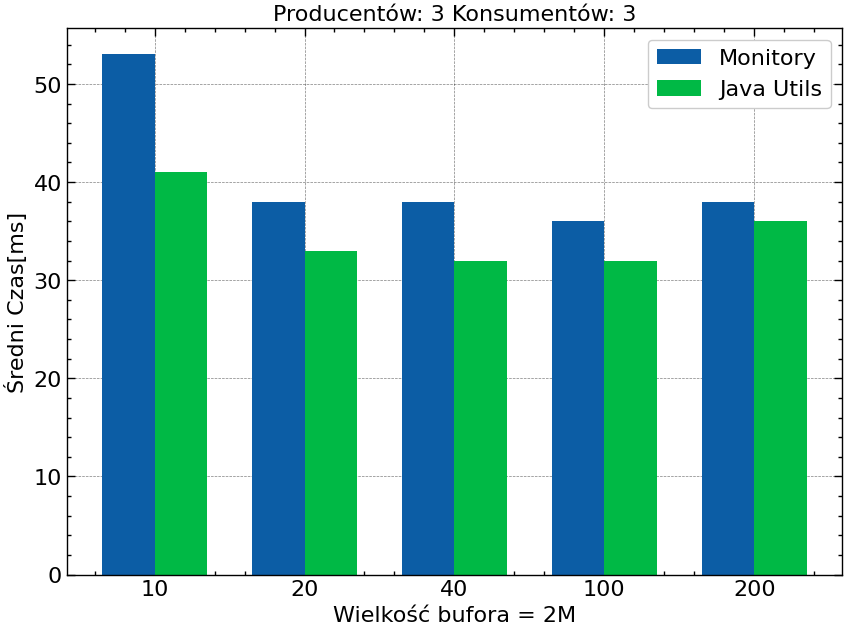
\includegraphics[width=12cm]{./m3_n3.png}
\end{center}

\begin{center}
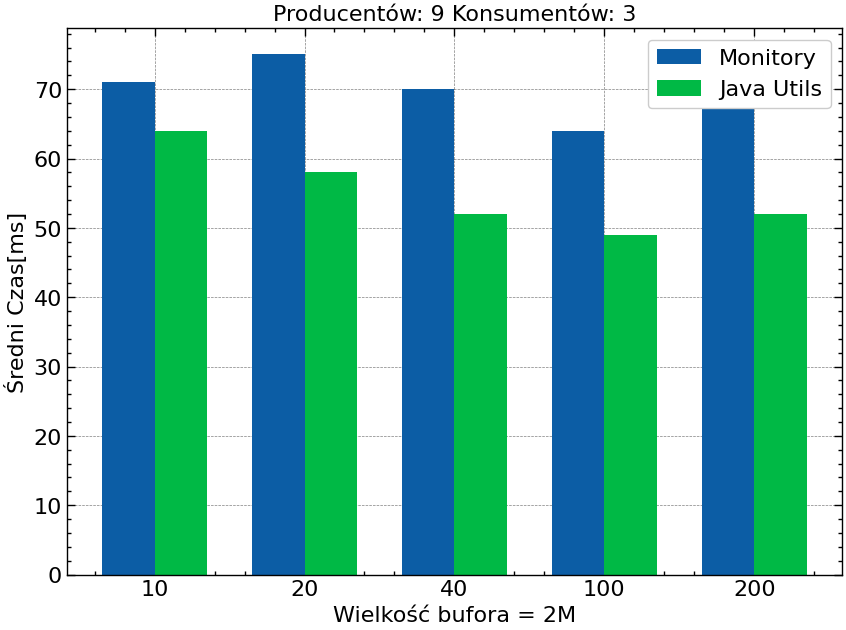
\includegraphics[width=12cm]{./m9_n3.png}
\end{center}

\begin{center}
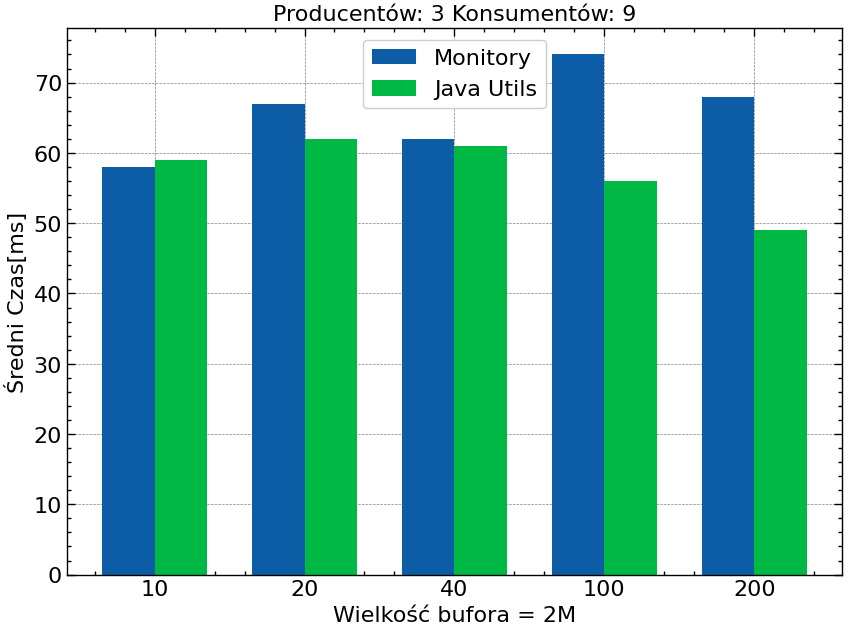
\includegraphics[width=12cm]{./m3_n9.png}
\end{center}

\begin{center}
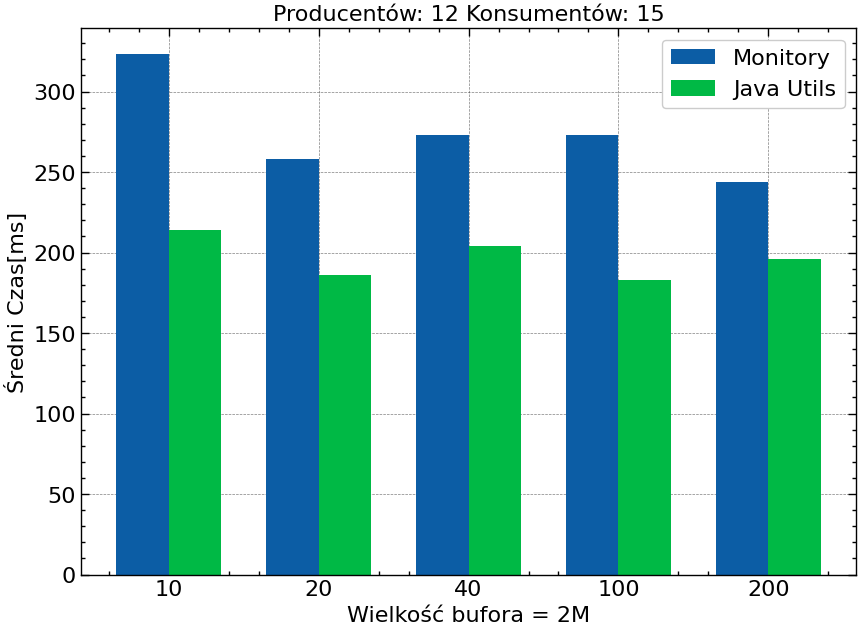
\includegraphics[width=12cm]{./m12_n15.png}
\end{center}

\begin{center}
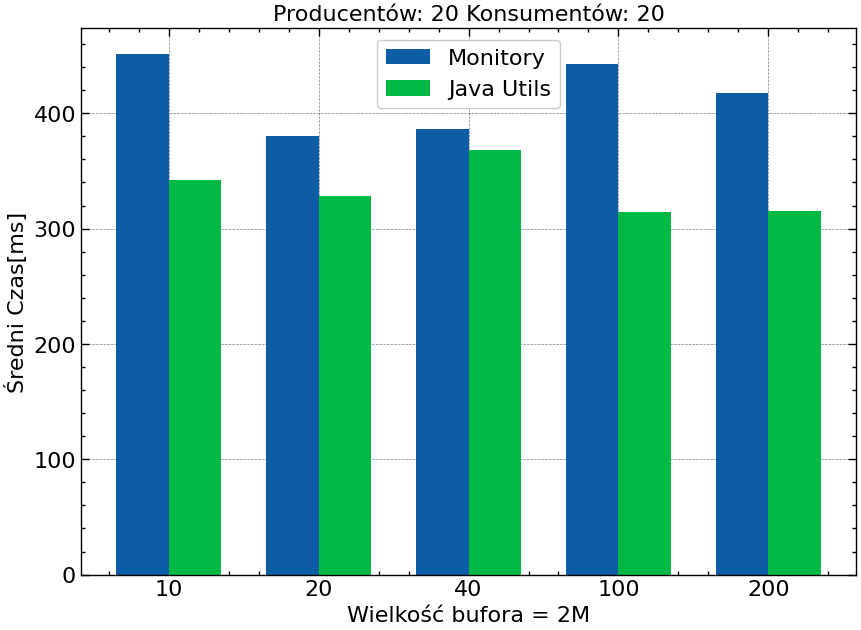
\includegraphics[width=12cm]{./m20_n20.png}
\end{center}

\begin{center}
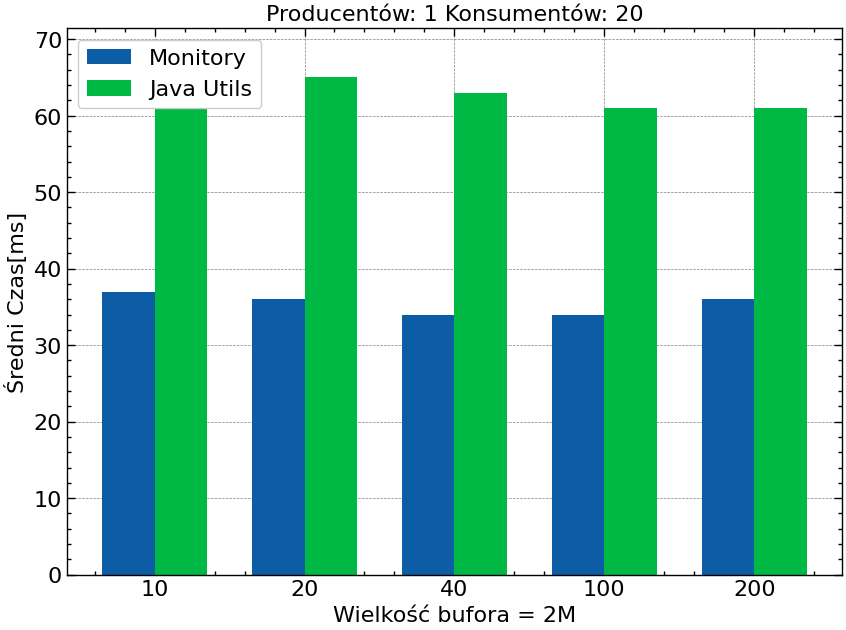
\includegraphics[width=12cm]{./m1_n20.png}
\end{center}

\begin{center}
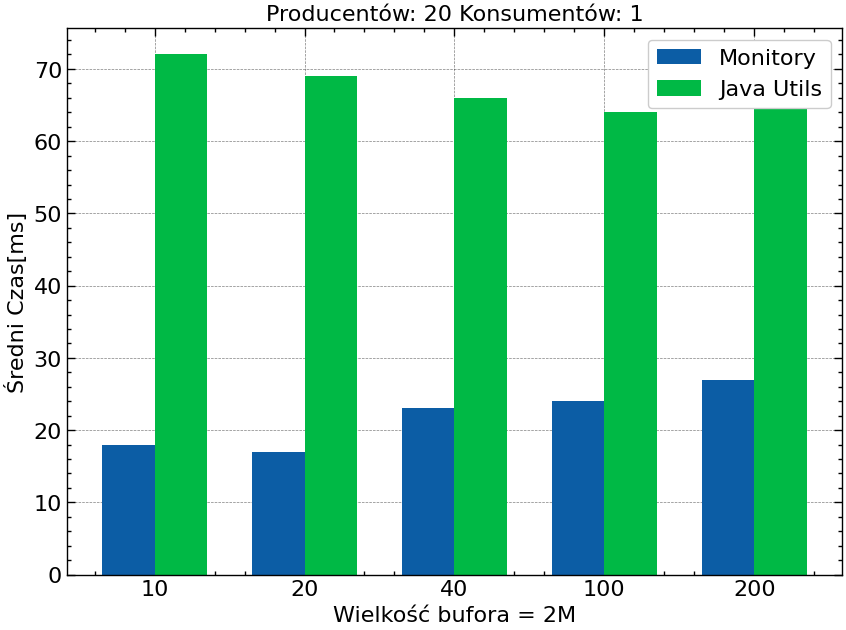
\includegraphics[width=12cm]{./m20_n1.png}
\end{center}

Widzimy, że wersja bufora korzystająca z \texttt{Java Concurrency Utilities} jest szybsza
niż wersja korzystająca z \texttt{monitorów} w większości przypadków.
Przyśpieszenie zapewne wynika z faktu, że \texttt{Condition} pozwala na bardziej precyzyjne
kontrolowanie przebudzeń wątków.
To co jest ciekawe, to fakt, że w skrajnych przydatkach, gdzie mamy zaledwie
jednego producenta lub konsumenta, to wersja korzystająca z monitorów jest szybsza.
Oznacza to, że badając wydajność współbieżnych programów, warto zwrócić uwagę na
skrajne przypadki, jeżeli uważamy, że mogą wystąpić w naszym programie.

Warto zwórócić uwagę, na to że biblioteka \texttt{Java Concurrency Utilities}
zawiera wiele innych mechanizmów, które nie zostały użyte w tym zadaniu.
Możliwe, że zastosowanie innych mechanizmów pozwoliłoby na jeszcze większe przyspieszenie.
\section*{Bibliografia}
\label{sec:orgfc66afa}
\begin{itemize}
\item Bill Venners: \emph{Inside the Java Virtual Machine Chapter 20}
\item \href{https://docs.oracle.com/javase/1.5.0/docs/guide/concurrency/overview.html}{Java Concurrency Utilities}
\item \href{https://docs.oracle.com/javase/1.5.0/docs/api/java/util/concurrent/locks/Condition.html}{Java Concurrency Utilities - Condition}
\item \href{https://docs.oracle.com/javase/1.5.0/docs/api/java/util/concurrent/locks/ReentrantLock.html}{Java Concurrency Utilities - ReentrantLock}
\end{itemize}
\end{document}
